\clearpage
\section{Experiment: Position-Angle}

Cleveland and McGill measure human perception to the ratios of positions and angles through comparisons on bar charts and pie charts~\cite{cleveland_mcgill}. We create rasterized images following Cleveland and McGill's proposed encoding and investigate computational perception of our networks (Figure~\ref{fig:teaser}). These have five bar or pie sectors representing numbers which add to 100, where each is greater than three and smaller than 39. One required change is in the minimal differences between the values: Cleveland and McGill create stimuli where the differences between each number are greater than $0.1$. However, as our networks only take $100\times100$ pixel images as input, we can only minimally represent a difference of $1$ pixel.

Cleveland and McGill ask participants to estimate the ratio of the four smaller bars or sectors to the known and marked largest bar or sector. As such, we mark the largest quantity of the five in each visualization with a single pixel dot, then ask our networks to perform multiple regression and produce the four ratio estimates. Since the position of the largest element changes, we generate the targets such that the largest element is marked with 1 and the smaller elements follow counter-clockwise for the pie chart and to the right for the bar chart. Each of the bar and pie chart visualizations has $878,520$ possible permutations.

% To be successful, the networks essentially first have to find the marked quantity, have the `rolling' encoding figured out, and then estimate the quantities properly.  -> JT: I don't want to prescribe how the network must solve the task. There are other ways to solve it, and this might not be how the network solves the problem.

%\begin{figure}[t]
%	  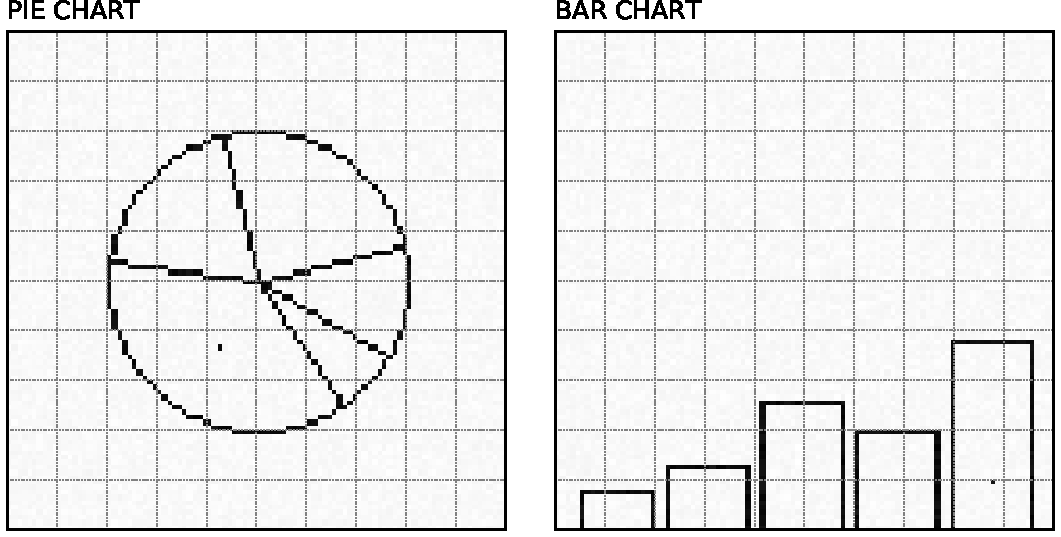
\includegraphics[width=\linewidth]{figure3_overview}
%  \caption{\textbf{Position-Angle Experiment.} We create rasterized visualizations of pie charts and bar charts to follow Cleveland and McGill's position-angle experiment. The experimental task involves the judgement of different encoded values in comparison to the largest encoded values. The pie chart (left) and the bar chart (right) visualize the same data point. In their paper, Cleveland and McGill report less errors using bar charts.}
%	\label{fig:position_angle_experiment}
%\end{figure}
%\begin{table}[h]
%\centering
%\caption{\textbf{Position-Angle Experiment.} We create rasterized visualizations of pie charts and bar charts to follow Cleveland and McGill's position-angle experiment. The experimental task involves the judgement of different encoded values in comparison to the largest encoded values. The pie chart and the bar chart visualize the same data point. In their paper, Cleveland and McGill report less errors using bar charts.}
%\resizebox{\linewidth}{!}{
%\begin{tabular}{lllr}
%	\toprule
%	\multicolumn{2}{l}{~} & ~ & Permutations\\
%
%	\midrule
%	\raisebox{-.85\height}{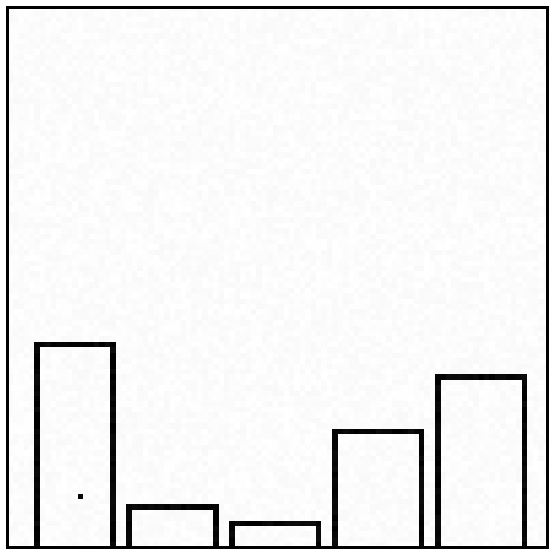
\includegraphics[width=.5in]{figure3_Bar_Chart.pdf}} & \makecell[tl]{Type 1: \emph{Bar Chart}\\~~~Perceptual Task: \emph{Position}\\~ \\~ \\} &~& \makecell[tr]{~\\ $878,520$}\\
%
%
%	\midrule
%	\raisebox{-.85\height}{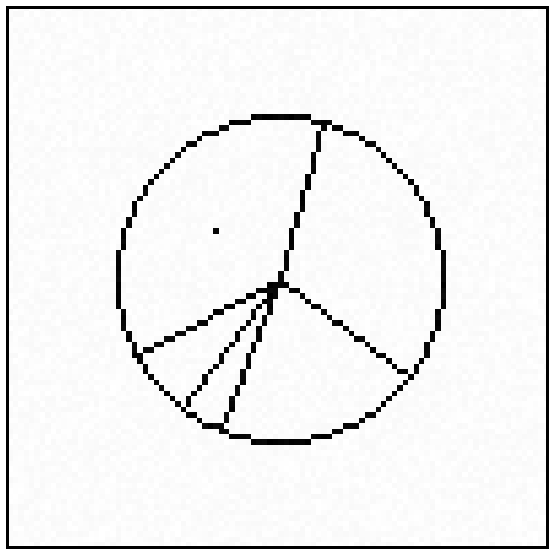
\includegraphics[width=.5in]{figure3_Pie_Chart.pdf}} & \makecell[tl]{Type 2: \emph{Pie Chart}\\~~~Perceptual Task: \emph{Angle}\\~ \\~ \\} &~& \makecell[tr]{~\\ $878,520$}\\
%
%
%	\bottomrule
%\end{tabular}
%}
%\label{tab:pos_angle_parameters}
%\end{table}

\subsection{Hypotheses}

\begin{hypolist}
	\item \textbf{H2.1} \textbf{Computed perceptual accuracy will be higher for bar charts than pie charts.} Cleveland and McGill report that position judgements are almost twice as accurate (MLAE) as angle judgements in humans. Following our ranking of elementary perceptual tasks (Table~\ref{tab:ranking}), we see that our networks also judge position encodings more accurately than angles, and so our networks will be able to more easily judge bar charts than pie charts.
	\item \textbf{H2.2} \textbf{Convolutional neural networks will learn to regress bar chart ratios faster than pie chart ratios in training.} This follows directly from H2.1.
\end{hypolist}

\subsection{Results}

\begin{figure}[t]
	\centering
	  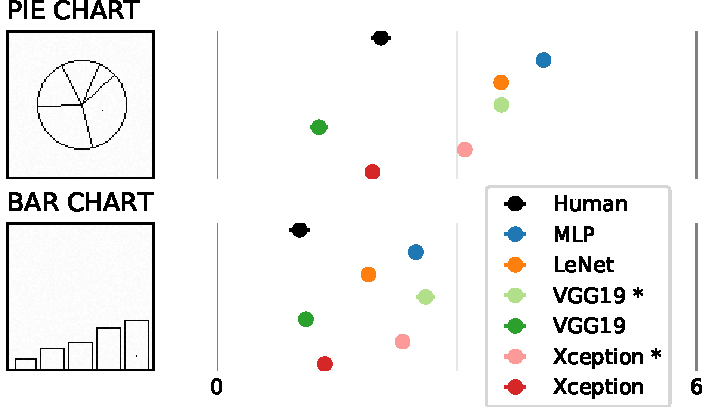
\includegraphics[width=\linewidth]{figure3_mlae_better_all.pdf}
  \caption{\textbf{Computational results of the position-angle experiment.} \textit{Left:} Our encodings of one data point as a pie chart and a bar chart. \textit{Right:} MLAE and 95\% confidence intervals for different networks. VGG19 * and Xception * are using ImageNet weights while all other networks were trained on the stimuli. We train all networks 12 times (4 times for VGG19 and Xception due to significantly longer training times). VGG19 * and Xception * use ImageNet weights. Our results align with Cleveland and McGill's human results, shown in black~\cite{cleveland_mcgill}.}
	\label{fig:figure3_mlae}
\end{figure}

% We evaluate over 56 runs for each condition \textit{visual encoding} (12 runs per network, but only 4 for VGG19 and Xception due to higher training times),

\noindent{\textbf{Perceptual Accuracy.}} Our networks are able to regress the task ratios for bar charts and pie charts (Fig.~\ref{fig:figure3_mlae}).  Cross-validation yields an average $MLAE=2.176$ ($SD=0.456$) for bar charts, and an average $MLAE=3.296$ ($SD=0.77$) for pie charts. This difference is statistically significant ($F_{1,110}=86.061, p<0.01$), and so we \textbf{accept H2.1}. 

Post hoc comparisons show that this holds for most networks: 
MLP for pie charts $4.09$ ($SD=0.027$) and for bar charts $2.494$ ($0.068$) is significant ($t_{22}=72.300,p<0.01$);
LeNet for pie charts $ 3.556 $ ($SD= 0.022 $) and for bar charts $ 1.902 $ ($SD= 0.08 $) is significant $t_{22}=66.111, p<0.01$;
VGG19 * with ImageNet weights for pie charts $ 3.561 $ ($SD= 0.047 $) and for bar charts $ 2.601 $ ($SD= 0.113 $) is significant $t_{22}=25.919,p<0.01$;
Xception * with ImageNet weights for pie charts  $ 3.094 $ ($SD= 0.046 $) and for bar charts $ 2.315 $ ($SD= 0.032 $) is significant $t_{22}=46.329,p<0.01$;
Xception from scratch for pie charts $ 1.939 $ ($SD= 0.1 $) and for bar charts $ 1.375 $ ($SD= 0.062 $) is significant $t_{22}=8.276,p<0.01$; but
the difference for VGG19 from scratch (pie charts $ 1.297 $ ($SD= 0.129 $), bar charts $ 1.153 $ ($SD= 0.09 $)) was not significant with $p<0.05$. 
This outcome is in line with the elementary perceptual task results (Table~\ref{tab:ranking}), where VGG19 was the most successful network, where networks trained from scratch were more performant, and where angle was more difficult to learn than position.
\\~\\
\noindent{\textbf{Training Efficiency.} We measure the MSE loss for all networks on previously-unseen validation data during training. We count a network as converged when this validation loss does not decrease after 10 sequential epochs. Figure~\ref{fig:figure3_val_loss} shows this MSE validation loss during the first twenty epochs for each condition, plotted across all cross-validation splits with overdrawn lines. The pie chart loss decreases more slowly, with the average loss over epochs being $0.052$ ($SD=0.015$) for pie charts and $0.037$ ($SD=0.018$) for bar charts. This difference is statistically significant ($F_{1,2238}=20.656, p<0.01$). Thus, we \textbf{accept H2.2}.
\\~\\
To all our networks, the bar chart is a superior visual encoding than a pie chart, in terms of accuracy and efficiency. Cleveland and McGill observe the same effect for accuracy during their human experiments.

% and conclude that the perceptual task of estimating position is easier for humans than the estimation of angles -> JT: Unless you have a direct quote, we're not putting words in their mouths. I couldn't find one in my brief look, but you might have one. If we do, then put a page number reference.

\begin{figure}[t]
	  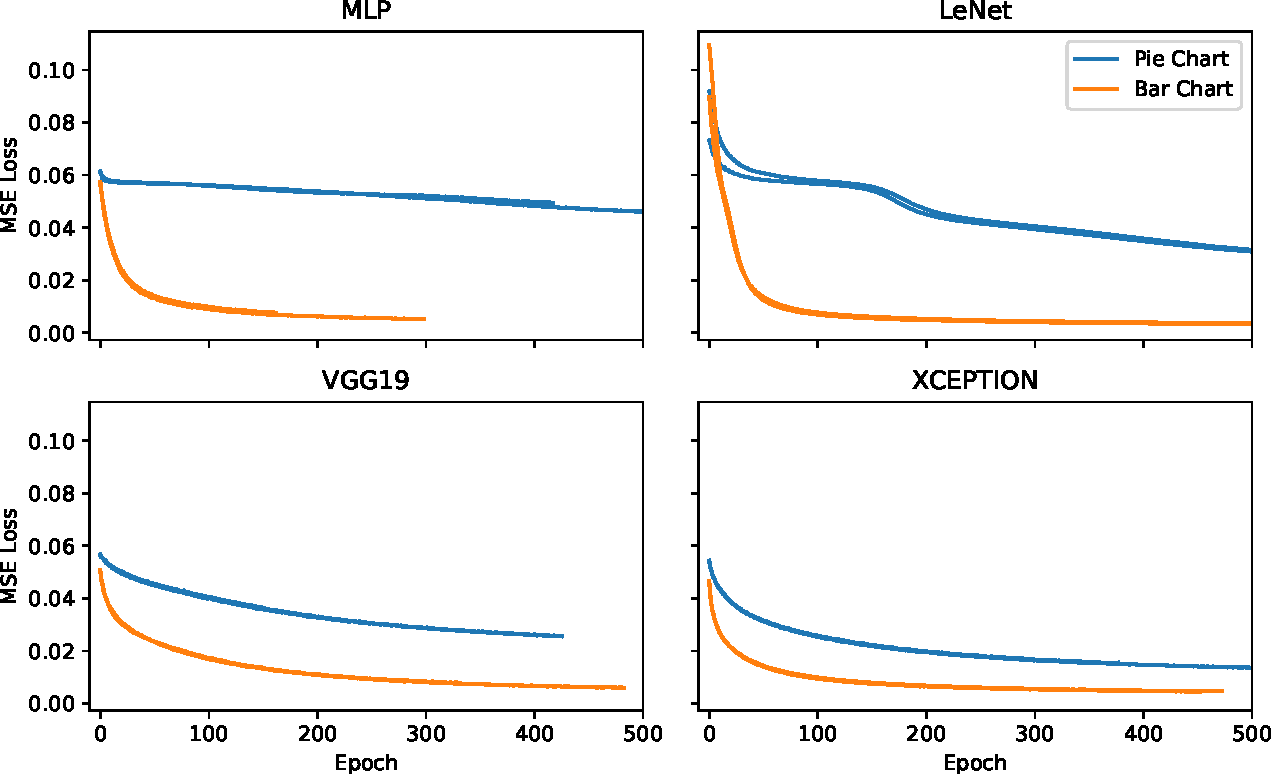
\includegraphics[width=\linewidth]{figure3_val_loss.pdf}
  \caption{\textbf{Training efficiency of the position-angle experiment.} Mean Squared Error (MSE) loss after each epoch during training, computed on previously-unseen validation data. We train all networks 12 times (4 times for VGG19 and Xception due to significantly longer training times). VGG19 * and Xception * use ImageNet weights. All networks converge faster when learning bar charts.}
	\label{fig:figure3_val_loss}
\end{figure}

